\documentclass{ximera}  

%\usepackage{todonotes}
%\usepackage{mathtools} %% Required for wide table Curl and Greens
%\usepackage{cuted} %% Required for wide table Curl and Greens
\newcommand{\todo}{}

\usepackage{esint} % for \oiint
\ifxake%%https://math.meta.stackexchange.com/questions/9973/how-do-you-render-a-closed-surface-double-integral
\renewcommand{\oiint}{{\large\bigcirc}\kern-1.56em\iint}
\fi


\graphicspath{
  {./}
  {jpg}
  {ximeraTutorial/}
  {basicPhilosophy/}
  {functionsOfSeveralVariables/}
  {normalVectors/}
  {lagrangeMultipliers/}
  {vectorFields/}
  {greensTheorem/}
  {shapeOfThingsToCome/}
  {dotProducts/}
  {partialDerivativesAndTheGradientVector/}
  {../productAndQuotientRules/exercises/}
  {../motionAndPathsInSpace/exercises/}
  {../normalVectors/exercisesParametricPlots/}
  {../continuityOfFunctionsOfSeveralVariables/exercises/}
  {../partialDerivativesAndTheGradientVector/exercises/}
  {../directionalDerivativeAndChainRule/exercises/}
  {../commonCoordinates/exercisesCylindricalCoordinates/}
  {../commonCoordinates/exercisesSphericalCoordinates/}
  {../greensTheorem/exercisesCurlAndLineIntegrals/}
  {../greensTheorem/exercisesDivergenceAndLineIntegrals/}
  {../shapeOfThingsToCome/exercisesDivergenceTheorem/}
  {../greensTheorem/}
  {../shapeOfThingsToCome/}
  {../separableDifferentialEquations/exercises/}
  {vectorFields/}
}

\newcommand{\mooculus}{\textsf{\textbf{MOOC}\textnormal{\textsf{ULUS}}}}

\usepackage{tkz-euclide}\usepackage{tikz}
\usepackage{tikz-cd}
\usetikzlibrary{arrows}
\tikzset{>=stealth,commutative diagrams/.cd,
  arrow style=tikz,diagrams={>=stealth}} %% cool arrow head
\tikzset{shorten <>/.style={ shorten >=#1, shorten <=#1 } } %% allows shorter vectors

\usetikzlibrary{backgrounds} %% for boxes around graphs
\usetikzlibrary{shapes,positioning}  %% Clouds and stars
\usetikzlibrary{matrix} %% for matrix
\usepgfplotslibrary{polar} %% for polar plots
\usepgfplotslibrary{fillbetween} %% to shade area between curves in TikZ
\usetkzobj{all}
\usepackage[makeroom]{cancel} %% for strike outs
%\usepackage{mathtools} %% for pretty underbrace % Breaks Ximera
%\usepackage{multicol}
\usepackage{pgffor} %% required for integral for loops



%% http://tex.stackexchange.com/questions/66490/drawing-a-tikz-arc-specifying-the-center
%% Draws beach ball
\tikzset{pics/carc/.style args={#1:#2:#3}{code={\draw[pic actions] (#1:#3) arc(#1:#2:#3);}}}



\usepackage{array}
\setlength{\extrarowheight}{+.1cm}
\newdimen\digitwidth
\settowidth\digitwidth{9}
\def\divrule#1#2{
\noalign{\moveright#1\digitwidth
\vbox{\hrule width#2\digitwidth}}}





\newcommand{\RR}{\mathbb R}
\newcommand{\R}{\mathbb R}
\newcommand{\N}{\mathbb N}
\newcommand{\Z}{\mathbb Z}

\newcommand{\sagemath}{\textsf{SageMath}}


%\renewcommand{\d}{\,d\!}
\renewcommand{\d}{\mathop{}\!d}
\newcommand{\dd}[2][]{\frac{\d #1}{\d #2}}
\newcommand{\pp}[2][]{\frac{\partial #1}{\partial #2}}
\renewcommand{\l}{\ell}
\newcommand{\ddx}{\frac{d}{\d x}}

\newcommand{\zeroOverZero}{\ensuremath{\boldsymbol{\tfrac{0}{0}}}}
\newcommand{\inftyOverInfty}{\ensuremath{\boldsymbol{\tfrac{\infty}{\infty}}}}
\newcommand{\zeroOverInfty}{\ensuremath{\boldsymbol{\tfrac{0}{\infty}}}}
\newcommand{\zeroTimesInfty}{\ensuremath{\small\boldsymbol{0\cdot \infty}}}
\newcommand{\inftyMinusInfty}{\ensuremath{\small\boldsymbol{\infty - \infty}}}
\newcommand{\oneToInfty}{\ensuremath{\boldsymbol{1^\infty}}}
\newcommand{\zeroToZero}{\ensuremath{\boldsymbol{0^0}}}
\newcommand{\inftyToZero}{\ensuremath{\boldsymbol{\infty^0}}}



\newcommand{\numOverZero}{\ensuremath{\boldsymbol{\tfrac{\#}{0}}}}
\newcommand{\dfn}{\textbf}
%\newcommand{\unit}{\,\mathrm}
\newcommand{\unit}{\mathop{}\!\mathrm}
\newcommand{\eval}[1]{\bigg[ #1 \bigg]}
\newcommand{\seq}[1]{\left( #1 \right)}
\renewcommand{\epsilon}{\varepsilon}
\renewcommand{\phi}{\varphi}


\renewcommand{\iff}{\Leftrightarrow}

\DeclareMathOperator{\arccot}{arccot}
\DeclareMathOperator{\arcsec}{arcsec}
\DeclareMathOperator{\arccsc}{arccsc}
\DeclareMathOperator{\si}{Si}
\DeclareMathOperator{\scal}{scal}
\DeclareMathOperator{\sign}{sign}


%% \newcommand{\tightoverset}[2]{% for arrow vec
%%   \mathop{#2}\limits^{\vbox to -.5ex{\kern-0.75ex\hbox{$#1$}\vss}}}
\newcommand{\arrowvec}[1]{{\overset{\rightharpoonup}{#1}}}
%\renewcommand{\vec}[1]{\arrowvec{\mathbf{#1}}}
\renewcommand{\vec}[1]{{\overset{\boldsymbol{\rightharpoonup}}{\mathbf{#1}}}\hspace{0in}}

\newcommand{\point}[1]{\left(#1\right)} %this allows \vector{ to be changed to \vector{ with a quick find and replace
\newcommand{\pt}[1]{\mathbf{#1}} %this allows \vec{ to be changed to \vec{ with a quick find and replace
\newcommand{\Lim}[2]{\lim_{\point{#1} \to \point{#2}}} %Bart, I changed this to point since I want to use it.  It runs through both of the exercise and exerciseE files in limits section, which is why it was in each document to start with.

\DeclareMathOperator{\proj}{\mathbf{proj}}
\newcommand{\veci}{{\boldsymbol{\hat{\imath}}}}
\newcommand{\vecj}{{\boldsymbol{\hat{\jmath}}}}
\newcommand{\veck}{{\boldsymbol{\hat{k}}}}
\newcommand{\vecl}{\vec{\boldsymbol{\l}}}
\newcommand{\uvec}[1]{\mathbf{\hat{#1}}}
\newcommand{\utan}{\mathbf{\hat{t}}}
\newcommand{\unormal}{\mathbf{\hat{n}}}
\newcommand{\ubinormal}{\mathbf{\hat{b}}}

\newcommand{\dotp}{\bullet}
\newcommand{\cross}{\boldsymbol\times}
\newcommand{\grad}{\boldsymbol\nabla}
\newcommand{\divergence}{\grad\dotp}
\newcommand{\curl}{\grad\cross}
%\DeclareMathOperator{\divergence}{divergence}
%\DeclareMathOperator{\curl}[1]{\grad\cross #1}
\newcommand{\lto}{\mathop{\longrightarrow\,}\limits}

\renewcommand{\bar}{\overline}

\colorlet{textColor}{black}
\colorlet{background}{white}
\colorlet{penColor}{blue!50!black} % Color of a curve in a plot
\colorlet{penColor2}{red!50!black}% Color of a curve in a plot
\colorlet{penColor3}{red!50!blue} % Color of a curve in a plot
\colorlet{penColor4}{green!50!black} % Color of a curve in a plot
\colorlet{penColor5}{orange!80!black} % Color of a curve in a plot
\colorlet{penColor6}{yellow!70!black} % Color of a curve in a plot
\colorlet{fill1}{penColor!20} % Color of fill in a plot
\colorlet{fill2}{penColor2!20} % Color of fill in a plot
\colorlet{fillp}{fill1} % Color of positive area
\colorlet{filln}{penColor2!20} % Color of negative area
\colorlet{fill3}{penColor3!20} % Fill
\colorlet{fill4}{penColor4!20} % Fill
\colorlet{fill5}{penColor5!20} % Fill
\colorlet{gridColor}{gray!50} % Color of grid in a plot

\newcommand{\surfaceColor}{violet}
\newcommand{\surfaceColorTwo}{redyellow}
\newcommand{\sliceColor}{greenyellow}




\pgfmathdeclarefunction{gauss}{2}{% gives gaussian
  \pgfmathparse{1/(#2*sqrt(2*pi))*exp(-((x-#1)^2)/(2*#2^2))}%
}


%%%%%%%%%%%%%
%% Vectors
%%%%%%%%%%%%%

%% Simple horiz vectors
\renewcommand{\vector}[1]{\left\langle #1\right\rangle}


%% %% Complex Horiz Vectors with angle brackets
%% \makeatletter
%% \renewcommand{\vector}[2][ , ]{\left\langle%
%%   \def\nextitem{\def\nextitem{#1}}%
%%   \@for \el:=#2\do{\nextitem\el}\right\rangle%
%% }
%% \makeatother

%% %% Vertical Vectors
%% \def\vector#1{\begin{bmatrix}\vecListA#1,,\end{bmatrix}}
%% \def\vecListA#1,{\if,#1,\else #1\cr \expandafter \vecListA \fi}

%%%%%%%%%%%%%
%% End of vectors
%%%%%%%%%%%%%

%\newcommand{\fullwidth}{}
%\newcommand{\normalwidth}{}



%% makes a snazzy t-chart for evaluating functions
%\newenvironment{tchart}{\rowcolors{2}{}{background!90!textColor}\array}{\endarray}

%%This is to help with formatting on future title pages.
\newenvironment{sectionOutcomes}{}{}



%% Flowchart stuff
%\tikzstyle{startstop} = [rectangle, rounded corners, minimum width=3cm, minimum height=1cm,text centered, draw=black]
%\tikzstyle{question} = [rectangle, minimum width=3cm, minimum height=1cm, text centered, draw=black]
%\tikzstyle{decision} = [trapezium, trapezium left angle=70, trapezium right angle=110, minimum width=3cm, minimum height=1cm, text centered, draw=black]
%\tikzstyle{question} = [rectangle, rounded corners, minimum width=3cm, minimum height=1cm,text centered, draw=black]
%\tikzstyle{process} = [rectangle, minimum width=3cm, minimum height=1cm, text centered, draw=black]
%\tikzstyle{decision} = [trapezium, trapezium left angle=70, trapezium right angle=110, minimum width=3cm, minimum height=1cm, text centered, draw=black]


\title{Basic Parameters of Sinusoidal Signals}  
\author{Milica Markovic}
\outcome{Recognize the basic properties of sinusoidal functions and relate them to circuit analysis. Describe basic properties of sinusoidal functions. Compare and contrast phase with time-delay.}
\begin{document}  
\begin{abstract}  
Review of Sinusoidal Signals
\end{abstract}  
\maketitle

\section{Sinusoidal signal parameters}

Sinusoidal signals are essential in electrical engineering as we use them to analyze and test circuit performance. All periodic signals can be represented with sinusoidal signals of different amplitudes and phases using the Fourier series. 

A typical sinusoidal signal is shown in Figure \ref{sinusoid}. On the y-axis is the instantaneous value of the sinusoidal voltage, and on the x-axis is time. Instantaneous values of voltage change from -1V to 1V with time. We use the following parameters to characterize sinusoidal signals: peak amplitude, peak-to-peak, average, RMS, period, time-delay, and phase. We read peak amplitude, peak-to-peak, average, and RMS values, on the y-axis in Figure \ref{sinusoid}, whereas period, time delay, and phase on the x-axis.

\begin{figure}[htbp]
\begin{center}
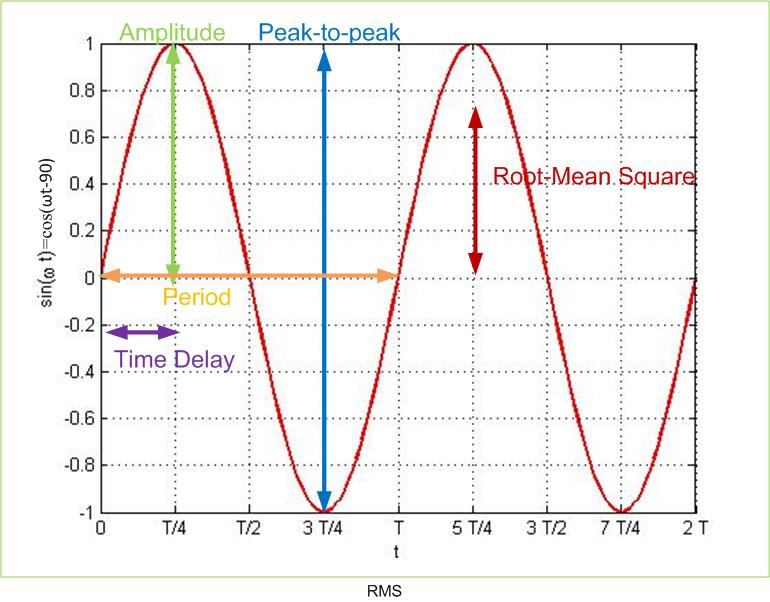
\includegraphics[scale=0.4]{jpg/sinusoid.jpg}
\caption{Vocabulary used in describing sinusoidal signals.}
\label{sinusoid}
\end{center}
\end{figure} 


\subsection{Parameters that are read on the y-axis.}

\begin{definition}
We read the peak amplitude on the y-axis from the average value of the signal (in this case, zero) to the signal's maximum value (in this case, 1). For signal shown in Figure \ref{sinusoid}, the peak  amplitude has a constant value of $V_p=1$. 
\end{definition}


\begin{definition}
The sinusoidal signal's instantaneous value varies from -1 to 1V, and its value depends on the x-axis. 

Compared to the instantaneous value, the peak amplitude is always constant, and it does not vary with time. 
\end{definition}

\begin{definition}
We measure peak-to-peak from the minimum value  (in this case, -1) to the maximum value (in this case, 1).  For signal shown in Figure \ref{sinusoid}, peak-to-peak voltage has a constant value of  $V_{pp}=2$.
\end{definition}

\begin{definition}
RMS or root-mean-square is defined as $v_{rms}=\frac{1}{T} \sqrt{\int_0^T v(t)^2 dt}$. For signal shown in Figure \ref{sinusoid}, and other sinusoidal signals of this form,  $v_{rms}=\frac{V_p}{\sqrt{2}}=\frac{1}{\sqrt{2}}=0.707$. Root mean square value is important because it represents the equivalent amount of DC power.
\end{definition}


\begin{definition}
Average value $v_{ave1}=\frac{1}{T} \int_0^T v(t) dt$. For the signal shown in Figure \ref{sinusoid}, the average value is $V_{ave1}=0$ because the function has the same area under the function in the positive and negative cycle. 
\end{definition}

\subsection{Parameters that are read on the x-axis.}

\begin{definition}
We can represent sinusoidal signals as a function of time, Figure \ref{sin}, or a function of angle, Figure \ref{sinPh}. Take a few minutes to see how the graphs are the same and how they are different.



\begin{figure}[htpb]
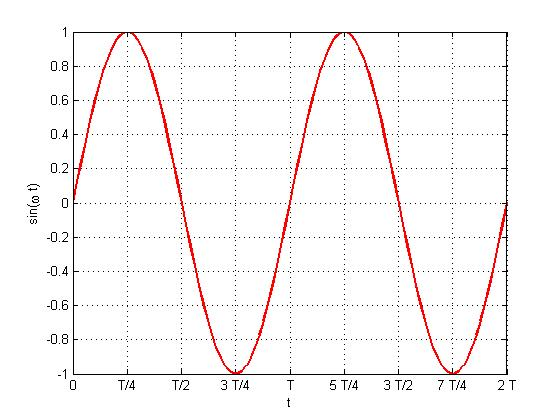
\includegraphics[scale=0.4]{jpg/cpef1.jpg}
\caption{$sin ( \omega t)$ as a function of time.} \label{sin}
\end{figure}




\begin{figure}[htpb]
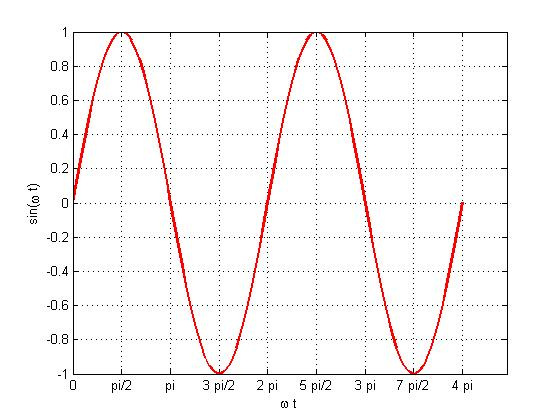
\includegraphics[scale=0.4]{jpg/cpef3.jpg}
\caption{Sinusoidal signal as a function of angle $\omega t$.}
\label{sinPh}
\end{figure}

\end{definition}


\begin{definition}
Period, T, is measured on the x-axis as the length of one full cycle of the sinusoidal signal. For signal shown in Figure \ref{sinusoid}, this value is $period=T$. 
\end{definition}

\begin{definition}
Frequency, f,  is defined as a reciprocal value of the period T, $f=\frac{1}{T}$. It represents how fast the signal is changing in time.  In Figure \ref{sinF1F2}, sinusoidal signals of two different frequencies f are given. 

\begin{figure}[htbp]
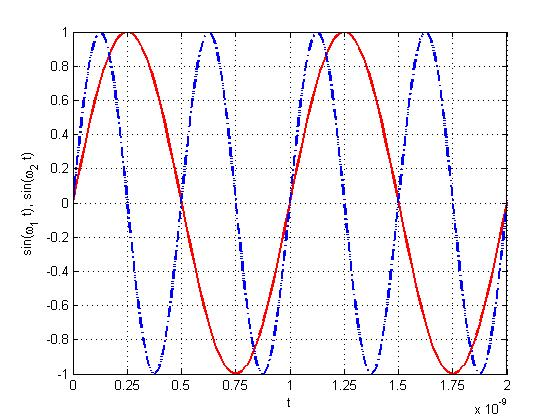
\includegraphics[scale=0.4]{jpg/cpef6.jpg}
\caption{Sinusoidal signals of different frequencies $sin ( \omega t)$}
\label{sinF1F2}
\end{figure}

\end{definition}

\begin{definition}
Time delay and phase represent the lag (or lead) of one function with respect to another in the time domain and frequency domain. For example, in Figure \ref{sinusoid}, function $ \cos(\omega t - 90^o)$ is time-delayed for $\tau = \frac{T}{4}$ with respect to $\cos (\omega t)$. To find the time delay from the phase, we look at how to represent the phase $90^o$ in terms of the product of frequency and time. Since in the sinusoidal signal expression $\cos (\omega t + \Theta)$  phase $\Theta$ is added to $\omega t$ term, the phase has the same units as $\omega t$, and can be represented as the product of $\omega \tau = \theta$, $\tau = \frac{\theta}{\omega}$, where $\tau$ represents the time delay.
\end{definition}









\begin{figure} [htbp]
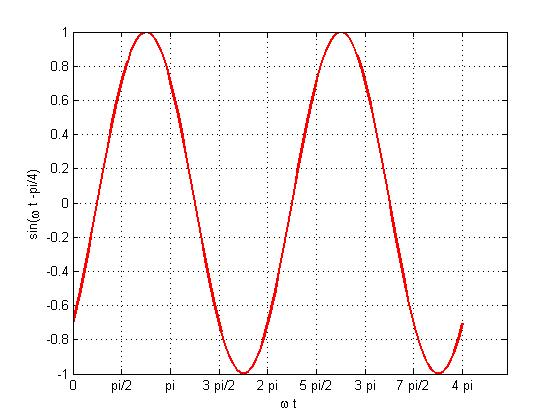
\includegraphics[scale=0.4]{jpg/cpef4.jpg}
\caption{Sinusoidal signal as a function of angle $\omega t$ with a phase shift of $-\pi/4$}
\label{sinMinus45Ph}
\end{figure}



\begin{question}  
Calculate the time-delay in nanoseconds that you would observe on an oscilloscope if the frequency of the signal is f=0.159\,GHz and the phase shift of the signal is $\theta=10^o$. \\
$ \frac{\theta}{2*\pi*f} = \answer{10}$  ns
\end{question} 

\begin{example}
Observe the three signals below, and change their amplitude and phase. Explain qualitatively how are the signals changing when we move the sliders?
\begin{center}  
\geogebra{w8r4epyh}{800}{600}  
\end{center} 
\end{example}





\end{document}



                                                                   



                                       




                                    















